\documentclass[twoside]{article}

% Packages required by doxygen
\usepackage{fixltx2e}
\usepackage{calc}
\usepackage{doxygen}
\usepackage{graphicx}
\usepackage[utf8]{inputenc}
\usepackage{makeidx}
\usepackage{multicol}
\usepackage{multirow}
\PassOptionsToPackage{warn}{textcomp}
\usepackage{textcomp}
\usepackage[nointegrals]{wasysym}
\usepackage[table]{xcolor}

% Font selection
\usepackage[T1]{fontenc}
\usepackage{mathptmx}
\usepackage[scaled=.90]{helvet}
\usepackage{courier}
\usepackage{amssymb}
\usepackage{sectsty}
\renewcommand{\familydefault}{\sfdefault}
\allsectionsfont{%
  \fontseries{bc}\selectfont%
  \color{darkgray}%
}
\renewcommand{\DoxyLabelFont}{%
  \fontseries{bc}\selectfont%
  \color{darkgray}%
}
\newcommand{\+}{\discretionary{\mbox{\scriptsize$\hookleftarrow$}}{}{}}

% Page & text layout
\usepackage[screen]{geometry}
\tolerance=750
\hfuzz=15pt
\hbadness=750
\setlength{\emergencystretch}{15pt}
\setlength{\parindent}{0cm}
\setlength{\parskip}{0.2cm}
\makeatletter
\renewcommand{\paragraph}{%
  \@startsection{paragraph}{4}{0ex}{-1.0ex}{1.0ex}{%
    \normalfont\normalsize\bfseries\SS@parafont%
  }%
}
\renewcommand{\subparagraph}{%
  \@startsection{subparagraph}{5}{0ex}{-1.0ex}{1.0ex}{%
    \normalfont\normalsize\bfseries\SS@subparafont%
  }%
}
\makeatother

% Headers & footers
\usepackage{fancyhdr}
\pagestyle{fancyplain}
\fancyhead[LE]{\fancyplain{}{\bfseries\thepage}}
\fancyhead[CE]{\fancyplain{}{}}
\fancyhead[RE]{\fancyplain{}{\bfseries\leftmark}}
\fancyhead[LO]{\fancyplain{}{\bfseries\rightmark}}
\fancyhead[CO]{\fancyplain{}{}}
\fancyhead[RO]{\fancyplain{}{\bfseries\thepage}}
\fancyfoot[LE]{\fancyplain{}{}}
\fancyfoot[CE]{\fancyplain{}{}}
\fancyfoot[RE]{\fancyplain{}{\bfseries\scriptsize Generated on Tue Oct 17 2017 14\+:35\+:42 for lab3 by Doxygen }}
\fancyfoot[LO]{\fancyplain{}{\bfseries\scriptsize Generated on Tue Oct 17 2017 14\+:35\+:42 for lab3 by Doxygen }}
\fancyfoot[CO]{\fancyplain{}{}}
\fancyfoot[RO]{\fancyplain{}{}}
\renewcommand{\footrulewidth}{0.4pt}
\renewcommand{\sectionmark}[1]{%
  \markright{\thesection\ #1}%
}

% Indices & bibliography
\usepackage{natbib}
\usepackage[titles]{tocloft}
\setcounter{tocdepth}{3}
\setcounter{secnumdepth}{5}
\makeindex

% Packages requested by user
\usepackage{titlesec}

% Hyperlinks (required, but should be loaded last)
\usepackage{ifpdf}
\ifpdf
  \usepackage[pdftex,pagebackref=true]{hyperref}
\else
  \usepackage[ps2pdf,pagebackref=true]{hyperref}
\fi
\hypersetup{%
  colorlinks=true,%
  linkcolor=blue,%
  citecolor=blue,%
  unicode%
}

% Custom commands
\newcommand{\clearemptydoublepage}{%
  \newpage{\pagestyle{empty}\cleardoublepage}%
}


\newcommand{\sectionbreak}{\clearpage}

\begin{document}

% Titlepage & ToC
\hypersetup{pageanchor=false,
             bookmarks=true,
             bookmarksnumbered=true,
             pdfencoding=unicode
            }
\pagenumbering{roman}
\begin{titlepage}
\vspace*{7cm}
\begin{center}%
{\Large lab3 }\\
\vspace*{1cm}
{\large Generated by Doxygen 1.8.8}\\
\vspace*{0.5cm}
{\small Tue Oct 17 2017 14:35:42}\\
\end{center}
\end{titlepage}
\tableofcontents
\pagenumbering{arabic}
\hypersetup{pageanchor=true}

%--- Begin generated contents ---
\section{Specification}
\label{Specification}
\hypertarget{Specification}{}
This is the English-\/\+Italian Dictionary program. The user can input an English word and the program will provide translation of the word. The current file the program uses to translate is and English to Italian Dictionary If the word that user enters is not in the program the the user can add the word into the dictionary by following the instructions given by the program.

Freatures\+:

1) The instructures are clear and concise to understand.

2) The ability to add words into the dictionary/program for later use.

3) Operator overlaoding to improve effiecncy of program. 
\section{Analysis}
\label{Analysis}
\hypertarget{Analysis}{}
When the user goes to the html page the program is already running. Here the user will be greeted by 6 options to select from. 5 of these options are sorting algorithms the other one is an option to see the times it takes for them to sort. When a sort is selected the page will load the name of the sort and then all the sorted info below it. Th fastest sort was quick sort which took less than a second. The slowest was bubble which varied from 40 seconds to 3 minutes. 
\section{Design}
\label{Design}
\hypertarget{Design}{}
Html was what we used to create the U\+I for this lab. T\+He translation program however was done in C++. We implemented a binary tree which basically allows us to store elements that can reference elements lower than it. Like tree -\/$>$ branches -\/$>$ twigs -\/$>$ leaves. The idea is that only an element of lower value can be stored in bottom of another element and lower is on the left and greater on the right. So in our lab a . was considered lower and a -\/ was conidered higher. This allowed us to reference letters within the tree very quickly. 
\section{Test}
\label{Test}
\hypertarget{Test}{}
 


 
\section{Class Index}
\subsection{Class List}
Here are the classes, structs, unions and interfaces with brief descriptions\+:\begin{DoxyCompactList}
\item\contentsline{section}{\hyperlink{structFRAGMENT}{F\+R\+A\+G\+M\+E\+N\+T} }{\pageref{structFRAGMENT}}{}
\item\contentsline{section}{\hyperlink{structMUSICELMT}{M\+U\+S\+I\+C\+E\+L\+M\+T} }{\pageref{structMUSICELMT}}{}
\item\contentsline{section}{\hyperlink{structNOTE}{N\+O\+T\+E} }{\pageref{structNOTE}}{}
\item\contentsline{section}{\hyperlink{structSTACK}{S\+T\+A\+C\+K} }{\pageref{structSTACK}}{}
\end{DoxyCompactList}

\section{File Index}
\subsection{File List}
Here is a list of all files with brief descriptions\+:\begin{DoxyCompactList}
\item\contentsline{section}{\hyperlink{addWords_8cpp}{add\+Words.\+cpp} }{\pageref{addWords_8cpp}}{}
\item\contentsline{section}{\hyperlink{foundWord_8cpp}{found\+Word.\+cpp} }{\pageref{foundWord_8cpp}}{}
\item\contentsline{section}{\hyperlink{lab_8cpp}{lab.\+cpp} }{\pageref{lab_8cpp}}{}
\item\contentsline{section}{\hyperlink{lab_8h}{lab.\+h} }{\pageref{lab_8h}}{}
\item\contentsline{section}{\hyperlink{loadDictionary_8cpp}{load\+Dictionary.\+cpp} }{\pageref{loadDictionary_8cpp}}{}
\item\contentsline{section}{\hyperlink{main_8cpp}{main.\+cpp} }{\pageref{main_8cpp}}{}
\end{DoxyCompactList}

\section{Class Documentation}
\hypertarget{structFRAGMENT}{\subsection{F\+R\+A\+G\+M\+E\+N\+T Struct Reference}
\label{structFRAGMENT}\index{F\+R\+A\+G\+M\+E\+N\+T@{F\+R\+A\+G\+M\+E\+N\+T}}
}


{\ttfamily \#include $<$lab.\+h$>$}

\subsubsection*{Public Attributes}
\begin{DoxyCompactItemize}
\item 
int \hyperlink{structFRAGMENT_a9a2c77dc5f1c259a9a063f8e6ae18724}{start}
\item 
int \hyperlink{structFRAGMENT_a3edee1f345e206cdc220b16d7d290018}{finish}
\end{DoxyCompactItemize}


\subsubsection{Member Data Documentation}
\hypertarget{structFRAGMENT_a3edee1f345e206cdc220b16d7d290018}{\index{F\+R\+A\+G\+M\+E\+N\+T@{F\+R\+A\+G\+M\+E\+N\+T}!finish@{finish}}
\index{finish@{finish}!F\+R\+A\+G\+M\+E\+N\+T@{F\+R\+A\+G\+M\+E\+N\+T}}
\paragraph[{finish}]{\setlength{\rightskip}{0pt plus 5cm}int F\+R\+A\+G\+M\+E\+N\+T\+::finish}}\label{structFRAGMENT_a3edee1f345e206cdc220b16d7d290018}
\hypertarget{structFRAGMENT_a9a2c77dc5f1c259a9a063f8e6ae18724}{\index{F\+R\+A\+G\+M\+E\+N\+T@{F\+R\+A\+G\+M\+E\+N\+T}!start@{start}}
\index{start@{start}!F\+R\+A\+G\+M\+E\+N\+T@{F\+R\+A\+G\+M\+E\+N\+T}}
\paragraph[{start}]{\setlength{\rightskip}{0pt plus 5cm}int F\+R\+A\+G\+M\+E\+N\+T\+::start}}\label{structFRAGMENT_a9a2c77dc5f1c259a9a063f8e6ae18724}


The documentation for this struct was generated from the following file\+:\begin{DoxyCompactItemize}
\item 
\hyperlink{lab_8h}{lab.\+h}\end{DoxyCompactItemize}

\hypertarget{structMUSICELMT}{\subsection{M\+U\+S\+I\+C\+E\+L\+M\+T Struct Reference}
\label{structMUSICELMT}\index{M\+U\+S\+I\+C\+E\+L\+M\+T@{M\+U\+S\+I\+C\+E\+L\+M\+T}}
}


{\ttfamily \#include $<$lab.\+h$>$}



Collaboration diagram for M\+U\+S\+I\+C\+E\+L\+M\+T\+:\nopagebreak
\begin{figure}[H]
\begin{center}
\leavevmode
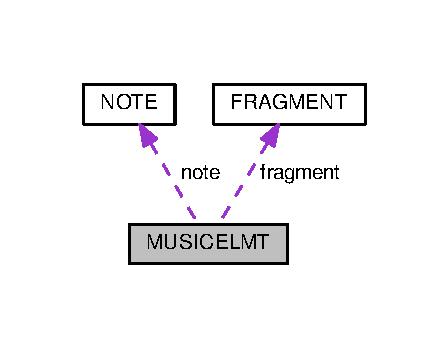
\includegraphics[width=215pt]{structMUSICELMT__coll__graph}
\end{center}
\end{figure}
\subsubsection*{Public Attributes}
\begin{DoxyCompactItemize}
\item 
\hyperlink{lab_8h_a41c816c739b4ab01c73879f01ae63880}{P\+L\+A\+Y} \hyperlink{structMUSICELMT_aa9a541d279b1a98b190c1968217ad37f}{type}
\item 
\begin{tabbing}
xx\=xx\=xx\=xx\=xx\=xx\=xx\=xx\=xx\=\kill
union \{\\
\>\hyperlink{structNOTE}{NOTE} \hyperlink{structMUSICELMT_a662fdb18330107012ed8902725b08e5c}{note}\\
\>\hyperlink{structFRAGMENT}{FRAGMENT} \hyperlink{structMUSICELMT_ae418bce8087e7510ad8563a87b4c1c63}{fragment}\\
\}; \\

\end{tabbing}\end{DoxyCompactItemize}


\subsubsection{Member Data Documentation}
\hypertarget{structMUSICELMT_af2898ea8d200b7d7c051d968d37e4788}{\paragraph[{"@1}]{\setlength{\rightskip}{0pt plus 5cm}union \{ ... \} }}\label{structMUSICELMT_af2898ea8d200b7d7c051d968d37e4788}
\hypertarget{structMUSICELMT_ae418bce8087e7510ad8563a87b4c1c63}{\index{M\+U\+S\+I\+C\+E\+L\+M\+T@{M\+U\+S\+I\+C\+E\+L\+M\+T}!fragment@{fragment}}
\index{fragment@{fragment}!M\+U\+S\+I\+C\+E\+L\+M\+T@{M\+U\+S\+I\+C\+E\+L\+M\+T}}
\paragraph[{fragment}]{\setlength{\rightskip}{0pt plus 5cm}{\bf F\+R\+A\+G\+M\+E\+N\+T} M\+U\+S\+I\+C\+E\+L\+M\+T\+::fragment}}\label{structMUSICELMT_ae418bce8087e7510ad8563a87b4c1c63}
\hypertarget{structMUSICELMT_a662fdb18330107012ed8902725b08e5c}{\index{M\+U\+S\+I\+C\+E\+L\+M\+T@{M\+U\+S\+I\+C\+E\+L\+M\+T}!note@{note}}
\index{note@{note}!M\+U\+S\+I\+C\+E\+L\+M\+T@{M\+U\+S\+I\+C\+E\+L\+M\+T}}
\paragraph[{note}]{\setlength{\rightskip}{0pt plus 5cm}{\bf N\+O\+T\+E} M\+U\+S\+I\+C\+E\+L\+M\+T\+::note}}\label{structMUSICELMT_a662fdb18330107012ed8902725b08e5c}
\hypertarget{structMUSICELMT_aa9a541d279b1a98b190c1968217ad37f}{\index{M\+U\+S\+I\+C\+E\+L\+M\+T@{M\+U\+S\+I\+C\+E\+L\+M\+T}!type@{type}}
\index{type@{type}!M\+U\+S\+I\+C\+E\+L\+M\+T@{M\+U\+S\+I\+C\+E\+L\+M\+T}}
\paragraph[{type}]{\setlength{\rightskip}{0pt plus 5cm}{\bf P\+L\+A\+Y} M\+U\+S\+I\+C\+E\+L\+M\+T\+::type}}\label{structMUSICELMT_aa9a541d279b1a98b190c1968217ad37f}


The documentation for this struct was generated from the following file\+:\begin{DoxyCompactItemize}
\item 
\hyperlink{lab_8h}{lab.\+h}\end{DoxyCompactItemize}

\hypertarget{structNOTE}{\subsection{N\+O\+T\+E Struct Reference}
\label{structNOTE}\index{N\+O\+T\+E@{N\+O\+T\+E}}
}


{\ttfamily \#include $<$lab.\+h$>$}

\subsubsection*{Public Attributes}
\begin{DoxyCompactItemize}
\item 
char \hyperlink{structNOTE_ae03dbb1306465fe61ec10da05fa5782e}{tone}
\item 
int \hyperlink{structNOTE_a258adf07267f95ab9630b33bad1b2fe2}{duration}
\end{DoxyCompactItemize}


\subsubsection{Member Data Documentation}
\hypertarget{structNOTE_a258adf07267f95ab9630b33bad1b2fe2}{\index{N\+O\+T\+E@{N\+O\+T\+E}!duration@{duration}}
\index{duration@{duration}!N\+O\+T\+E@{N\+O\+T\+E}}
\paragraph[{duration}]{\setlength{\rightskip}{0pt plus 5cm}int N\+O\+T\+E\+::duration}}\label{structNOTE_a258adf07267f95ab9630b33bad1b2fe2}
\hypertarget{structNOTE_ae03dbb1306465fe61ec10da05fa5782e}{\index{N\+O\+T\+E@{N\+O\+T\+E}!tone@{tone}}
\index{tone@{tone}!N\+O\+T\+E@{N\+O\+T\+E}}
\paragraph[{tone}]{\setlength{\rightskip}{0pt plus 5cm}char N\+O\+T\+E\+::tone}}\label{structNOTE_ae03dbb1306465fe61ec10da05fa5782e}


The documentation for this struct was generated from the following file\+:\begin{DoxyCompactItemize}
\item 
\hyperlink{lab_8h}{lab.\+h}\end{DoxyCompactItemize}

\hypertarget{structSTACK}{\subsection{S\+T\+A\+C\+K Struct Reference}
\label{structSTACK}\index{S\+T\+A\+C\+K@{S\+T\+A\+C\+K}}
}


{\ttfamily \#include $<$lab.\+h$>$}

\subsubsection*{Public Attributes}
\begin{DoxyCompactItemize}
\item 
int \hyperlink{structSTACK_ad10f9d8025122e8c82832d7a34c77e40}{size}
\item 
int $\ast$ \hyperlink{structSTACK_a6d512f82cbd75729347a293193039538}{buf}
\item 
int \hyperlink{structSTACK_a1b186cf876dace2f1e30fcbe260cad9a}{sp}
\end{DoxyCompactItemize}


\subsubsection{Member Data Documentation}
\hypertarget{structSTACK_a6d512f82cbd75729347a293193039538}{\index{S\+T\+A\+C\+K@{S\+T\+A\+C\+K}!buf@{buf}}
\index{buf@{buf}!S\+T\+A\+C\+K@{S\+T\+A\+C\+K}}
\paragraph[{buf}]{\setlength{\rightskip}{0pt plus 5cm}int$\ast$ S\+T\+A\+C\+K\+::buf}}\label{structSTACK_a6d512f82cbd75729347a293193039538}
\hypertarget{structSTACK_ad10f9d8025122e8c82832d7a34c77e40}{\index{S\+T\+A\+C\+K@{S\+T\+A\+C\+K}!size@{size}}
\index{size@{size}!S\+T\+A\+C\+K@{S\+T\+A\+C\+K}}
\paragraph[{size}]{\setlength{\rightskip}{0pt plus 5cm}int S\+T\+A\+C\+K\+::size}}\label{structSTACK_ad10f9d8025122e8c82832d7a34c77e40}
\hypertarget{structSTACK_a1b186cf876dace2f1e30fcbe260cad9a}{\index{S\+T\+A\+C\+K@{S\+T\+A\+C\+K}!sp@{sp}}
\index{sp@{sp}!S\+T\+A\+C\+K@{S\+T\+A\+C\+K}}
\paragraph[{sp}]{\setlength{\rightskip}{0pt plus 5cm}int S\+T\+A\+C\+K\+::sp}}\label{structSTACK_a1b186cf876dace2f1e30fcbe260cad9a}


The documentation for this struct was generated from the following file\+:\begin{DoxyCompactItemize}
\item 
\hyperlink{lab_8h}{lab.\+h}\end{DoxyCompactItemize}

\section{File Documentation}
\hypertarget{create_8cpp}{\subsection{create.\+cpp File Reference}
\label{create_8cpp}\index{create.\+cpp@{create.\+cpp}}
}
{\ttfamily \#include \char`\"{}lab.\+h\char`\"{}}\\*
Include dependency graph for create.\+cpp\+:\nopagebreak
\begin{figure}[H]
\begin{center}
\leavevmode
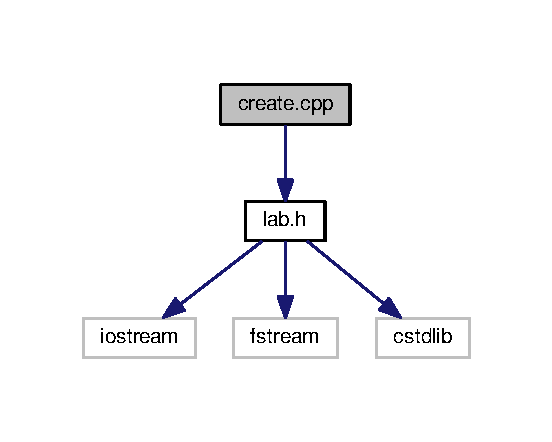
\includegraphics[width=265pt]{create_8cpp__incl}
\end{center}
\end{figure}
\subsubsection*{Functions}
\begin{DoxyCompactItemize}
\item 
\hyperlink{lab_8h_a32c27cc471df37f4fc818d65de0a56c4}{S\+T\+A\+T\+U\+S} \hyperlink{create_8cpp_abd657d26045a775f57a837427142cfbd}{Create} (\hyperlink{structSTACK}{S\+T\+A\+C\+K} \&stack, int size)
\end{DoxyCompactItemize}


\subsubsection{Function Documentation}
\hypertarget{create_8cpp_abd657d26045a775f57a837427142cfbd}{\index{create.\+cpp@{create.\+cpp}!Create@{Create}}
\index{Create@{Create}!create.\+cpp@{create.\+cpp}}
\paragraph[{Create}]{\setlength{\rightskip}{0pt plus 5cm}{\bf S\+T\+A\+T\+U\+S} Create (
\begin{DoxyParamCaption}
\item[{{\bf S\+T\+A\+C\+K} \&}]{stack, }
\item[{int}]{size}
\end{DoxyParamCaption}
)}}\label{create_8cpp_abd657d26045a775f57a837427142cfbd}

\begin{DoxyCode}
4 \{
5     stack.\hyperlink{structSTACK_a6d512f82cbd75729347a293193039538}{buf} = \textcolor{keyword}{new} \textcolor{keywordtype}{int}[size];
6     \textcolor{keywordflow}{if} (!stack.\hyperlink{structSTACK_a6d512f82cbd75729347a293193039538}{buf})
7         \textcolor{keywordflow}{return} \hyperlink{lab_8h_a32c27cc471df37f4fc818d65de0a56c4aecedb56d1405a60c6069f4a0139bdec5}{FAILED};
8     stack.\hyperlink{structSTACK_ad10f9d8025122e8c82832d7a34c77e40}{size} = size;
9     stack.\hyperlink{structSTACK_a1b186cf876dace2f1e30fcbe260cad9a}{sp} = 0;
10     \textcolor{keywordflow}{return} \hyperlink{lab_8h_a32c27cc471df37f4fc818d65de0a56c4a2bc49ec37d6a5715dd23e85f1ff5bb59}{OK};
11 \}
\end{DoxyCode}

\hypertarget{destroy_8cpp}{\subsection{destroy.\+cpp File Reference}
\label{destroy_8cpp}\index{destroy.\+cpp@{destroy.\+cpp}}
}
{\ttfamily \#include \char`\"{}lab.\+h\char`\"{}}\\*
Include dependency graph for destroy.\+cpp\+:\nopagebreak
\begin{figure}[H]
\begin{center}
\leavevmode
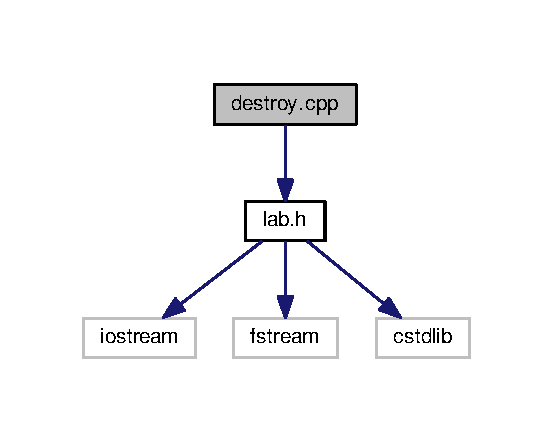
\includegraphics[width=265pt]{destroy_8cpp__incl}
\end{center}
\end{figure}
\subsubsection*{Functions}
\begin{DoxyCompactItemize}
\item 
\hyperlink{lab_8h_a32c27cc471df37f4fc818d65de0a56c4}{S\+T\+A\+T\+U\+S} \hyperlink{destroy_8cpp_a74b9065a1e9ff8a9f20a1234743d443c}{Destroy} (\hyperlink{structSTACK}{S\+T\+A\+C\+K} \&stack)
\end{DoxyCompactItemize}


\subsubsection{Function Documentation}
\hypertarget{destroy_8cpp_a74b9065a1e9ff8a9f20a1234743d443c}{\index{destroy.\+cpp@{destroy.\+cpp}!Destroy@{Destroy}}
\index{Destroy@{Destroy}!destroy.\+cpp@{destroy.\+cpp}}
\paragraph[{Destroy}]{\setlength{\rightskip}{0pt plus 5cm}{\bf S\+T\+A\+T\+U\+S} Destroy (
\begin{DoxyParamCaption}
\item[{{\bf S\+T\+A\+C\+K} \&}]{stack}
\end{DoxyParamCaption}
)}}\label{destroy_8cpp_a74b9065a1e9ff8a9f20a1234743d443c}
This is the function that destroys the stack. it taks in stack as the parameter 
\begin{DoxyCode}
7 \{
8     \textcolor{keyword}{delete} [] stack.\hyperlink{structSTACK_a6d512f82cbd75729347a293193039538}{buf};
9 \}
\end{DoxyCode}

\hypertarget{lab_8h}{\subsection{lab.\+h File Reference}
\label{lab_8h}\index{lab.\+h@{lab.\+h}}
}
{\ttfamily \#include $<$fstream$>$}\\*
{\ttfamily \#include $<$iostream$>$}\\*
{\ttfamily \#include $<$string$>$}\\*
Include dependency graph for lab.\+h\+:\nopagebreak
\begin{figure}[H]
\begin{center}
\leavevmode
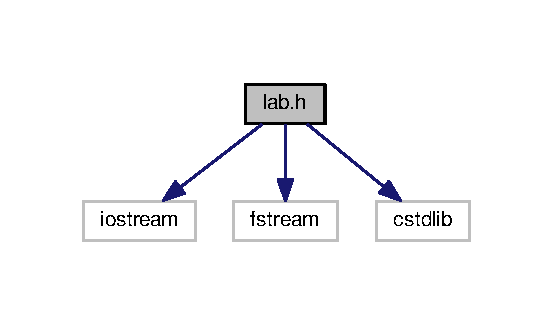
\includegraphics[width=261pt]{lab_8h__incl}
\end{center}
\end{figure}
This graph shows which files directly or indirectly include this file\+:\nopagebreak
\begin{figure}[H]
\begin{center}
\leavevmode
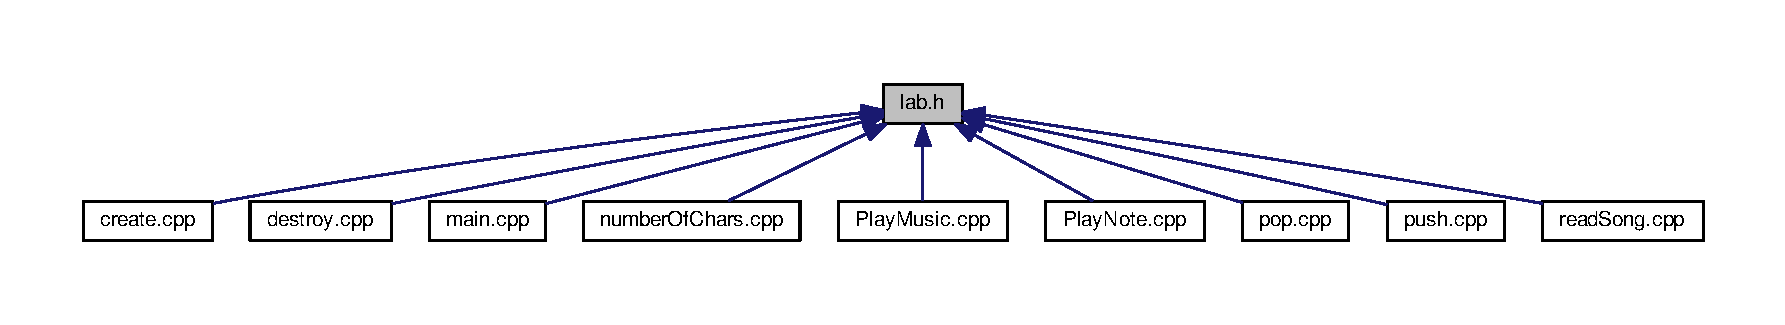
\includegraphics[width=350pt]{lab_8h__dep__incl}
\end{center}
\end{figure}
\subsubsection*{Classes}
\begin{DoxyCompactItemize}
\item 
struct \hyperlink{structNODE}{N\+O\+D\+E}
\begin{DoxyCompactList}\small\item\em City Structure. \end{DoxyCompactList}\end{DoxyCompactItemize}
\subsubsection*{Enumerations}
\begin{DoxyCompactItemize}
\item 
enum \hyperlink{lab_8h_a32c27cc471df37f4fc818d65de0a56c4}{S\+T\+A\+T\+U\+S} \{ \hyperlink{lab_8h_a32c27cc471df37f4fc818d65de0a56c4aecedb56d1405a60c6069f4a0139bdec5}{F\+A\+I\+L\+E\+D}, 
\hyperlink{lab_8h_a32c27cc471df37f4fc818d65de0a56c4a2bc49ec37d6a5715dd23e85f1ff5bb59}{O\+K}
 \}
\end{DoxyCompactItemize}
\subsubsection*{Functions}
\begin{DoxyCompactItemize}
\item 
\hyperlink{lab_8h_a32c27cc471df37f4fc818d65de0a56c4}{S\+T\+A\+T\+U\+S} \hyperlink{lab_8h_a578b73f866dc4391d05ca0219f892495}{insert} (\hyperlink{structNODE}{N\+O\+D\+E} $\ast$\&head, std\+::string city)
\begin{DoxyCompactList}\small\item\em Insert inserts a new node at the beginning of the list. \end{DoxyCompactList}\item 
\hyperlink{lab_8h_a32c27cc471df37f4fc818d65de0a56c4}{S\+T\+A\+T\+U\+S} \hyperlink{lab_8h_abf14767ea6c86eb593d6f87fe77267e7}{insertinorder} (\hyperlink{structNODE}{N\+O\+D\+E} $\ast$\&head, std\+::string city)
\item 
\hyperlink{lab_8h_a32c27cc471df37f4fc818d65de0a56c4}{S\+T\+A\+T\+U\+S} \hyperlink{lab_8h_a9eb7dfa9761b11c255d499765ea70b75}{builddirectly} (\hyperlink{structNODE}{N\+O\+D\+E} $\ast$\&head, string cities)
\item 
void \hyperlink{lab_8h_a67a34562a85e577c0921c5d65c22decc}{destroylist} (\hyperlink{structNODE}{N\+O\+D\+E} $\ast$head)
\item 
void \hyperlink{lab_8h_a6b2cb293574fc5dc8d7a4897cacea16f}{displaylist} (\hyperlink{structNODE}{N\+O\+D\+E} $\ast$head)
\item 
\hyperlink{structNODE}{N\+O\+D\+E} $\ast$ \hyperlink{lab_8h_afd6087490d82489b892a41298eba4e60}{loadlist} (std\+::string filename)
\end{DoxyCompactItemize}


\subsubsection{Enumeration Type Documentation}
\hypertarget{lab_8h_a32c27cc471df37f4fc818d65de0a56c4}{\index{lab.\+h@{lab.\+h}!S\+T\+A\+T\+U\+S@{S\+T\+A\+T\+U\+S}}
\index{S\+T\+A\+T\+U\+S@{S\+T\+A\+T\+U\+S}!lab.\+h@{lab.\+h}}
\paragraph[{S\+T\+A\+T\+U\+S}]{\setlength{\rightskip}{0pt plus 5cm}enum {\bf S\+T\+A\+T\+U\+S}}}\label{lab_8h_a32c27cc471df37f4fc818d65de0a56c4}
\begin{Desc}
\item[Enumerator]\par
\begin{description}
\index{F\+A\+I\+L\+E\+D@{F\+A\+I\+L\+E\+D}!lab.\+h@{lab.\+h}}\index{lab.\+h@{lab.\+h}!F\+A\+I\+L\+E\+D@{F\+A\+I\+L\+E\+D}}\item[{\em 
\hypertarget{lab_8h_a32c27cc471df37f4fc818d65de0a56c4aecedb56d1405a60c6069f4a0139bdec5}{F\+A\+I\+L\+E\+D}\label{lab_8h_a32c27cc471df37f4fc818d65de0a56c4aecedb56d1405a60c6069f4a0139bdec5}
}]\index{O\+K@{O\+K}!lab.\+h@{lab.\+h}}\index{lab.\+h@{lab.\+h}!O\+K@{O\+K}}\item[{\em 
\hypertarget{lab_8h_a32c27cc471df37f4fc818d65de0a56c4a2bc49ec37d6a5715dd23e85f1ff5bb59}{O\+K}\label{lab_8h_a32c27cc471df37f4fc818d65de0a56c4a2bc49ec37d6a5715dd23e85f1ff5bb59}
}]\end{description}
\end{Desc}

\begin{DoxyCode}
7 \{\hyperlink{lab_8h_a32c27cc471df37f4fc818d65de0a56c4aecedb56d1405a60c6069f4a0139bdec5}{FAILED}, \hyperlink{lab_8h_a32c27cc471df37f4fc818d65de0a56c4a2bc49ec37d6a5715dd23e85f1ff5bb59}{OK}\};
\end{DoxyCode}


\subsubsection{Function Documentation}
\hypertarget{lab_8h_a9eb7dfa9761b11c255d499765ea70b75}{\index{lab.\+h@{lab.\+h}!builddirectly@{builddirectly}}
\index{builddirectly@{builddirectly}!lab.\+h@{lab.\+h}}
\paragraph[{builddirectly}]{\setlength{\rightskip}{0pt plus 5cm}{\bf S\+T\+A\+T\+U\+S} builddirectly (
\begin{DoxyParamCaption}
\item[{{\bf N\+O\+D\+E} $\ast$\&}]{head, }
\item[{string}]{cities}
\end{DoxyParamCaption}
)}}\label{lab_8h_a9eb7dfa9761b11c255d499765ea70b75}

\begin{DoxyCode}
5 \{
6     \textcolor{keywordtype}{string} city;
7     \hyperlink{structNODE}{NODE}* tail; 
8     ifstream ifs(\textcolor{stringliteral}{"cities"});
9     \textcolor{keywordflow}{if} (! ifs) 
10     \textcolor{keywordflow}{return} \hyperlink{lab_8h_a32c27cc471df37f4fc818d65de0a56c4aecedb56d1405a60c6069f4a0139bdec5}{FAILED};
11     
12 \textcolor{keywordflow}{while}(ifs >> city) \{
13     \hyperlink{structNODE}{NODE} *newnode = \textcolor{keyword}{new} \hyperlink{structNODE}{NODE};
14     \textcolor{keywordflow}{if}(!newnode)
15     \textcolor{keywordflow}{return} \hyperlink{lab_8h_a32c27cc471df37f4fc818d65de0a56c4aecedb56d1405a60c6069f4a0139bdec5}{FAILED};
16     
17     newnode->\hyperlink{structNODE_a76c9a9603778b363e65bfe84da4bd72e}{city} = city;
18     
19     newnode->\hyperlink{structNODE_a078472e8ab2d2fe38e052f5c2a425618}{next} = 0;
20     
21      \textcolor{keywordflow}{if}(!tail) \{
22         head = newnode;\}
23     \textcolor{keywordflow}{else} \{
24         tail->\hyperlink{structNODE_a078472e8ab2d2fe38e052f5c2a425618}{next} = newnode;
25     \}
26     tail = newnode;
27     
28 \}
29 \}
\end{DoxyCode}
\hypertarget{lab_8h_a67a34562a85e577c0921c5d65c22decc}{\index{lab.\+h@{lab.\+h}!destroylist@{destroylist}}
\index{destroylist@{destroylist}!lab.\+h@{lab.\+h}}
\paragraph[{destroylist}]{\setlength{\rightskip}{0pt plus 5cm}void destroylist (
\begin{DoxyParamCaption}
\item[{{\bf N\+O\+D\+E} $\ast$}]{head}
\end{DoxyParamCaption}
)}}\label{lab_8h_a67a34562a85e577c0921c5d65c22decc}

\begin{DoxyParams}[1]{Parameters}
\mbox{\tt in}  & {\em head} & This is the only parameter the function takes.\\
\hline
\end{DoxyParams}
This function completely destroys the list.


\begin{DoxyImage}
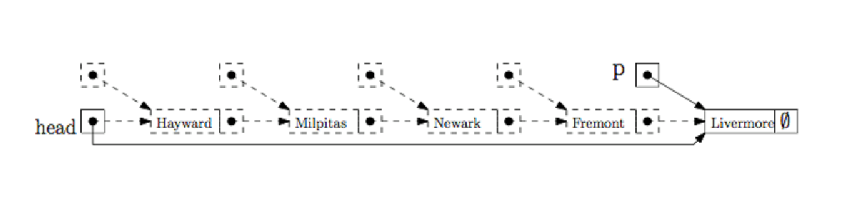
\includegraphics{destroylist1}
\caption{Linked List}
\end{DoxyImage}
 As you can see that this function points the head at the node and then deletes it severing the tie to the list 
\begin{DoxyCode}
14 \{
15     \hyperlink{structNODE}{NODE}* node;
16     \textcolor{keywordflow}{for}(node = head; node; node = node->\hyperlink{structNODE_a078472e8ab2d2fe38e052f5c2a425618}{next})
17     \{
18         cout << \textcolor{stringliteral}{"deleting: "}
19             << node->\hyperlink{structNODE_a76c9a9603778b363e65bfe84da4bd72e}{city} << std::endl;
20         \hyperlink{structNODE}{NODE}* tmp = head->\hyperlink{structNODE_a078472e8ab2d2fe38e052f5c2a425618}{next};
21         \textcolor{keyword}{delete} head;
22         head = tmp;
23         
24     \}
25     
26 \}
\end{DoxyCode}
\hypertarget{lab_8h_a6b2cb293574fc5dc8d7a4897cacea16f}{\index{lab.\+h@{lab.\+h}!displaylist@{displaylist}}
\index{displaylist@{displaylist}!lab.\+h@{lab.\+h}}
\paragraph[{displaylist}]{\setlength{\rightskip}{0pt plus 5cm}void displaylist (
\begin{DoxyParamCaption}
\item[{{\bf N\+O\+D\+E} $\ast$}]{head}
\end{DoxyParamCaption}
)}}\label{lab_8h_a6b2cb293574fc5dc8d7a4897cacea16f}

\begin{DoxyParams}[1]{Parameters}
\mbox{\tt in}  & {\em head} & This fucntion only takes a pointer as an argument.\\
\hline
\end{DoxyParams}
This function displays/traverses the list This is what a linked list looks like to a user It traverses the list without manipulating any pointers. See the comments for further deatils 
\begin{DoxyCode}
11 \{
12     \textcolor{comment}{//first we set the node pointer equal to the head pointer}
13     \textcolor{comment}{//Then while node exists this loop continues}
14     \textcolor{comment}{//Then we set the pointer equal to the next pointer }
15 
16     \textcolor{keywordflow}{for}(\hyperlink{structNODE}{NODE}* node = head; node; node = node->\hyperlink{structNODE_a078472e8ab2d2fe38e052f5c2a425618}{next})
17     \textcolor{comment}{//This displays the data within the node}
18     cout << node->city << endl;
19 \}
\end{DoxyCode}
\hypertarget{lab_8h_a578b73f866dc4391d05ca0219f892495}{\index{lab.\+h@{lab.\+h}!insert@{insert}}
\index{insert@{insert}!lab.\+h@{lab.\+h}}
\paragraph[{insert}]{\setlength{\rightskip}{0pt plus 5cm}{\bf S\+T\+A\+T\+U\+S} insert (
\begin{DoxyParamCaption}
\item[{{\bf N\+O\+D\+E} $\ast$\&}]{head, }
\item[{std\+::string}]{city}
\end{DoxyParamCaption}
)}}\label{lab_8h_a578b73f866dc4391d05ca0219f892495}


Insert inserts a new node at the beginning of the list. 


\begin{DoxyParams}[1]{Parameters}
\mbox{\tt in,out}  & {\em head} & The head of the linked list \\
\hline
\mbox{\tt in}  & {\em city} & The data in the node being inserted \\
\hline
\end{DoxyParams}
\begin{DoxyReturn}{Returns}
A S\+T\+A\+T\+U\+S indicating if Insert was successful of not
\end{DoxyReturn}

\begin{DoxyParams}[1]{Parameters}
\mbox{\tt in,out}  & {\em head} & The head of the linked list \\
\hline
\mbox{\tt in}  & {\em city} & The data in the node being inserted \\
\hline
\end{DoxyParams}
\begin{DoxyReturn}{Returns}
A S\+T\+A\+T\+U\+S indicating if Insert was successful of not 
\begin{DoxyImage}
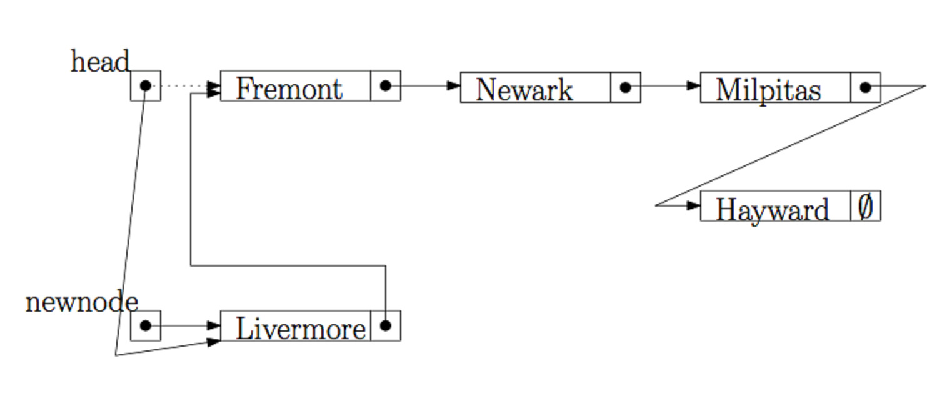
\includegraphics{insert}
\caption{Linked List}
\end{DoxyImage}
 
\end{DoxyReturn}

\begin{DoxyCode}
11 \{
12     \textcolor{comment}{//city = "Dublin"}
13     \hyperlink{structNODE}{NODE} *newnode;
14     
15     \textcolor{comment}{// Allocate a new node:}
16     
17     newnode = \textcolor{keyword}{new} \hyperlink{structNODE}{NODE};
18     \textcolor{keywordflow}{if} (!newnode)
19         \textcolor{keywordflow}{return} \hyperlink{lab_8h_a32c27cc471df37f4fc818d65de0a56c4aecedb56d1405a60c6069f4a0139bdec5}{FAILED}; 
20     \textcolor{comment}{//copy the info into the new node:}
21     
22     newnode->\hyperlink{structNODE_a76c9a9603778b363e65bfe84da4bd72e}{city} = city;
23     
24     \textcolor{comment}{//Link the new node to the list:}
25     
26     newnode->\hyperlink{structNODE_a078472e8ab2d2fe38e052f5c2a425618}{next} = head;
27     head = newnode; 
28     
29     \textcolor{keywordflow}{return} \hyperlink{lab_8h_a32c27cc471df37f4fc818d65de0a56c4a2bc49ec37d6a5715dd23e85f1ff5bb59}{OK}; 
30 \}
\end{DoxyCode}
\hypertarget{lab_8h_abf14767ea6c86eb593d6f87fe77267e7}{\index{lab.\+h@{lab.\+h}!insertinorder@{insertinorder}}
\index{insertinorder@{insertinorder}!lab.\+h@{lab.\+h}}
\paragraph[{insertinorder}]{\setlength{\rightskip}{0pt plus 5cm}{\bf S\+T\+A\+T\+U\+S} insertinorder (
\begin{DoxyParamCaption}
\item[{{\bf N\+O\+D\+E} $\ast$\&}]{head, }
\item[{std\+::string}]{city}
\end{DoxyParamCaption}
)}}\label{lab_8h_abf14767ea6c86eb593d6f87fe77267e7}

\begin{DoxyParams}[1]{Parameters}
\mbox{\tt in}  & {\em head,string} & This functions takes in the head and a string which is whatever city the user defines\\
\hline
\end{DoxyParams}
This function inserts a city into the list in a specific order.


\begin{DoxyImage}
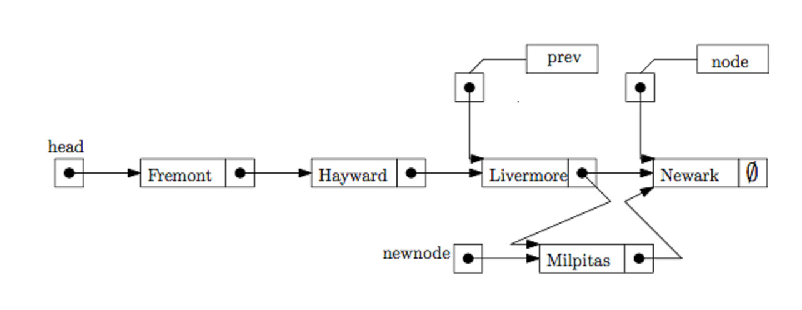
\includegraphics{insertinorder}
\caption{Linked List}
\end{DoxyImage}
 This shows how the pointers previous and next work as they traverse the list looking for a place to insert. Once it does it changes the pointers to add the value into the list 
\begin{DoxyCode}
16 \{
17     \hyperlink{structNODE}{NODE} *newnode;
18      \textcolor{comment}{// Allocate a new node:}
19      
20     newnode = \textcolor{keyword}{new} \hyperlink{structNODE}{NODE};
21     \textcolor{keywordflow}{if} (!newnode)
22         \textcolor{keywordflow}{return} \hyperlink{lab_8h_a32c27cc471df37f4fc818d65de0a56c4aecedb56d1405a60c6069f4a0139bdec5}{FAILED};
23         
24     \textcolor{comment}{// Copy the info into newnode:}
25     
26     newnode->\hyperlink{structNODE_a76c9a9603778b363e65bfe84da4bd72e}{city} = city;
27     
28     \textcolor{comment}{// LINK newnode to the list:}
29     \textcolor{comment}{// a) Find the right place to insert newnode (between "prev" and "node":}
30     
31     \hyperlink{structNODE}{NODE} *\hyperlink{structNODE}{NODE} = head, *prev = 0;
32     \textcolor{keywordflow}{while} (NODE && NODE->\hyperlink{structNODE_a76c9a9603778b363e65bfe84da4bd72e}{city} <= city) \{
33         \textcolor{comment}{//node->city <= city}
34     prev = NODE;        \textcolor{comment}{//advance node and prev}
35     NODE = NODE->\hyperlink{structNODE_a078472e8ab2d2fe38e052f5c2a425618}{next};
36 \}
37     \textcolor{comment}{// b) Link newnode between prev and node}
38     
39     newnode->\hyperlink{structNODE_a078472e8ab2d2fe38e052f5c2a425618}{next} = NODE; \textcolor{comment}{//append node to newnode}
40     \textcolor{keywordflow}{if} (prev)
41         prev->\hyperlink{structNODE_a078472e8ab2d2fe38e052f5c2a425618}{next} = newnode; \textcolor{comment}{//Insert after "prev"}
42     \textcolor{keywordflow}{else} 
43         head = newnode; \textcolor{comment}{//No prev: make new node the new head}
44         
45         \textcolor{keywordflow}{return} \hyperlink{lab_8h_a32c27cc471df37f4fc818d65de0a56c4a2bc49ec37d6a5715dd23e85f1ff5bb59}{OK};
46     \}
\end{DoxyCode}
\hypertarget{lab_8h_afd6087490d82489b892a41298eba4e60}{\index{lab.\+h@{lab.\+h}!loadlist@{loadlist}}
\index{loadlist@{loadlist}!lab.\+h@{lab.\+h}}
\paragraph[{loadlist}]{\setlength{\rightskip}{0pt plus 5cm}{\bf N\+O\+D\+E}$\ast$ loadlist (
\begin{DoxyParamCaption}
\item[{std\+::string}]{filename}
\end{DoxyParamCaption}
)}}\label{lab_8h_afd6087490d82489b892a41298eba4e60}
This function loads the dictionary into a linked list it takes the filename \char`\"{}cities\char`\"{} and loads that as cities the variable Then it uses the insert function to create the list after the head pointer. Then at the end it returns head so that we can use it in other functions. 
\begin{DoxyCode}
10 \{
11     \hyperlink{structNODE}{NODE}* head = 0; \textcolor{comment}{// this is where we declare the head as null to create the list}
12     std::ifstream ifs(filename.c\_str());
13     \textcolor{keywordtype}{string} city;
14     \textcolor{keywordflow}{while}(ifs >> city) 
15         \textcolor{keywordflow}{if}(\hyperlink{insert_8cpp_a578b73f866dc4391d05ca0219f892495}{insert}(head,city) == \hyperlink{lab_8h_a32c27cc471df37f4fc818d65de0a56c4aecedb56d1405a60c6069f4a0139bdec5}{FAILED})
16          cerr << \textcolor{stringliteral}{"error on insert\(\backslash\)n"};
17          
18     \textcolor{keywordflow}{return} head;
19 \}
\end{DoxyCode}

\hypertarget{main_8cpp}{\subsection{main.\+cpp File Reference}
\label{main_8cpp}\index{main.\+cpp@{main.\+cpp}}
}
{\ttfamily \#include \char`\"{}lab.\+h\char`\"{}}\\*
Include dependency graph for main.\+cpp\+:\nopagebreak
\begin{figure}[H]
\begin{center}
\leavevmode
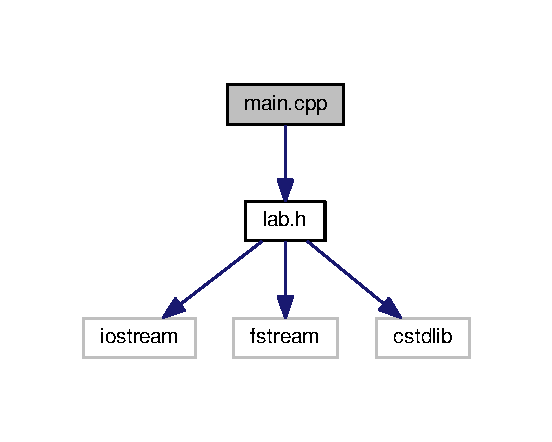
\includegraphics[width=264pt]{main_8cpp__incl}
\end{center}
\end{figure}
\subsubsection*{Functions}
\begin{DoxyCompactItemize}
\item 
int \hyperlink{main_8cpp_ae66f6b31b5ad750f1fe042a706a4e3d4}{main} ()
\end{DoxyCompactItemize}


\subsubsection{Function Documentation}
\hypertarget{main_8cpp_ae66f6b31b5ad750f1fe042a706a4e3d4}{\index{main.\+cpp@{main.\+cpp}!main@{main}}
\index{main@{main}!main.\+cpp@{main.\+cpp}}
\paragraph[{main}]{\setlength{\rightskip}{0pt plus 5cm}int main (
\begin{DoxyParamCaption}
{}
\end{DoxyParamCaption}
)}}\label{main_8cpp_ae66f6b31b5ad750f1fe042a706a4e3d4}
This is main function of the project. Contains the three fucntions (loaddictionary, foundwords, addwords) See comments for better understanding 
\begin{DoxyCode}
11 \{
12     vector<Entry> dict;
13     \textcolor{keywordtype}{string} word; \textcolor{comment}{// user inputs word}
14     \textcolor{keywordtype}{string} translation; \textcolor{comment}{// outputs translation}
15     \textcolor{keywordtype}{bool} ok, quit;
16     
17     ok = \hyperlink{lab_8h_ac18625e34f66c3bc052e07dfb0d3d219}{loaddictionary}(\textcolor{stringliteral}{"dict.dat"}, dict);
18     \textcolor{keywordflow}{if} (!ok) \{
19         cout << \textcolor{stringliteral}{" **** Cannot load Dictionary ***** \(\backslash\)n"};
20         \textcolor{keywordflow}{return} 1; \textcolor{comment}{//ERROR}
21     \}
22     
23     
24     \textcolor{keywordtype}{string} line;
25     
26  ifstream inpfile(\textcolor{stringliteral}{"dict.dat"}); \textcolor{comment}{//opening file again so that once updated }
27     \textcolor{keywordflow}{if} (!inpfile) \textcolor{keywordflow}{return} \textcolor{keyword}{false}; \textcolor{comment}{//the new information can be called without restarting the program}
28     
29     getline(inpfile, line);
30     cout << line << endl;
31     cout << \textcolor{stringliteral}{"Program by Samuel Jothimuthu"} <<endl;
32 
33     quit = \textcolor{keyword}{false};
34     \textcolor{keywordflow}{while} (!quit) \{ \textcolor{comment}{//iteration control structure}
35         \hyperlink{lab_8h_ac18625e34f66c3bc052e07dfb0d3d219}{loaddictionary}(\textcolor{stringliteral}{"dict.dat"}, dict);
36 
37         \textcolor{keywordtype}{string} choice; \textcolor{comment}{//simple choice of yes or no }
38         \textcolor{keywordtype}{string} newtran; \textcolor{comment}{//new translation for word user enters}
39         \textcolor{keywordtype}{string} inputstring; \textcolor{comment}{// the full string that will be appened to the file "dict.dat"}
40         cout << \textcolor{stringliteral}{"Enter a word or 'q' to quit ==> "};
41         cin >> word;
42         cin.ignore(80, \textcolor{charliteral}{'\(\backslash\)n'}); \textcolor{comment}{//this allows the console argument to execute but skipping the line}
43         \textcolor{keywordflow}{if} (word == \textcolor{stringliteral}{"q"}) 
44             quit = \textcolor{keyword}{true};
45         \textcolor{keywordflow}{else} \textcolor{keywordflow}{if} (\hyperlink{foundWord_8cpp_ae41eba27837d0aeea84fb5c6824388db}{foundword}( dict, word, translation)) \textcolor{comment}{//function must return true}
46             cout << translation << \textcolor{stringliteral}{"\(\backslash\)n\(\backslash\)n"};
47         \textcolor{keywordflow}{else} \textcolor{comment}{//The selection control structure}
48            \{ cout << word << \textcolor{stringliteral}{" --not in the dictionary. \(\backslash\)n Would you like to add it? (y/n)\(\backslash\)n"};
49             cin >> choice;
50             \textcolor{keywordflow}{if} (choice == \textcolor{stringliteral}{"y"}) \{ \textcolor{comment}{//any other input does not work. }
51                 cout << \textcolor{stringliteral}{"What is the Italian translation for "} << word << \textcolor{stringliteral}{"?"} << endl;
52                 cin >> newtran;
53                 inputstring = word + \textcolor{stringliteral}{"\(\backslash\)t"} + newtran; \textcolor{comment}{// this builds the full string that the program can
       then call upon.}
54                 \hyperlink{addWords_8cpp_ab5aa985d3bd8d2b89a2d5f35f38fb868}{addwords}(\textcolor{stringliteral}{"dict.dat"}, inputstring); \textcolor{comment}{//runs the addwords function, adding it into the
       file.}
55                 \}
56         \}
57         \}
58         \textcolor{keywordflow}{return} 0;
59     \}
\end{DoxyCode}

\hypertarget{numberOfChars_8cpp}{\subsection{number\+Of\+Chars.\+cpp File Reference}
\label{numberOfChars_8cpp}\index{number\+Of\+Chars.\+cpp@{number\+Of\+Chars.\+cpp}}
}
{\ttfamily \#include \char`\"{}lab.\+h\char`\"{}}\\*
Include dependency graph for number\+Of\+Chars.\+cpp\+:\nopagebreak
\begin{figure}[H]
\begin{center}
\leavevmode
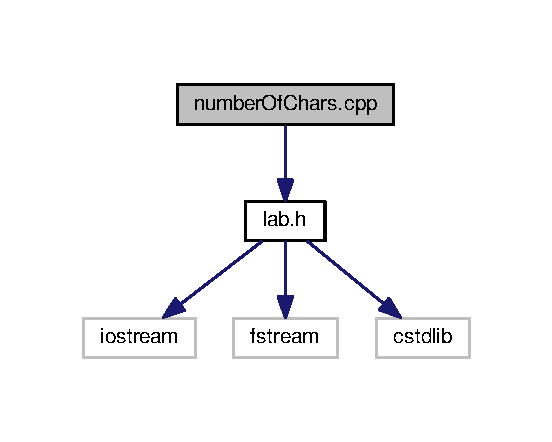
\includegraphics[width=265pt]{numberOfChars_8cpp__incl}
\end{center}
\end{figure}
\subsubsection*{Functions}
\begin{DoxyCompactItemize}
\item 
int \hyperlink{numberOfChars_8cpp_abc8df280a4f34fc23a2dd8b1b4a6cc41}{numberofchars} (std\+::ifstream \&f)
\end{DoxyCompactItemize}


\subsubsection{Function Documentation}
\hypertarget{numberOfChars_8cpp_abc8df280a4f34fc23a2dd8b1b4a6cc41}{\index{number\+Of\+Chars.\+cpp@{number\+Of\+Chars.\+cpp}!numberofchars@{numberofchars}}
\index{numberofchars@{numberofchars}!number\+Of\+Chars.\+cpp@{number\+Of\+Chars.\+cpp}}
\paragraph[{numberofchars}]{\setlength{\rightskip}{0pt plus 5cm}int numberofchars (
\begin{DoxyParamCaption}
\item[{std\+::ifstream \&}]{f}
\end{DoxyParamCaption}
)}}\label{numberOfChars_8cpp_abc8df280a4f34fc23a2dd8b1b4a6cc41}
This program counts the number of chareters in the abc notion 
\begin{DoxyCode}
6 \{
7     \textcolor{keywordtype}{int} n = 0;
8     \textcolor{comment}{//count characters}
9     \textcolor{keywordtype}{char} c;
10     \textcolor{keywordflow}{while}(f >> c)
11         n++;
12     \textcolor{keywordflow}{return} n;
13 \}
\end{DoxyCode}

\hypertarget{PlayMusic_8cpp}{\subsection{Play\+Music.\+cpp File Reference}
\label{PlayMusic_8cpp}\index{Play\+Music.\+cpp@{Play\+Music.\+cpp}}
}
{\ttfamily \#include \char`\"{}lab.\+h\char`\"{}}\\*
Include dependency graph for Play\+Music.\+cpp\+:\nopagebreak
\begin{figure}[H]
\begin{center}
\leavevmode
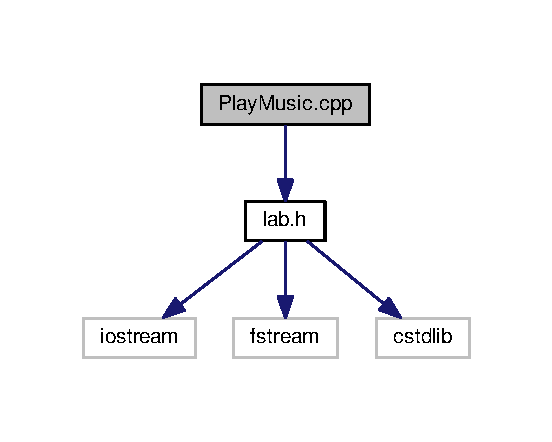
\includegraphics[width=265pt]{PlayMusic_8cpp__incl}
\end{center}
\end{figure}
\subsubsection*{Functions}
\begin{DoxyCompactItemize}
\item 
void \hyperlink{PlayMusic_8cpp_a678c8ab56091134ef699893df8a5f683}{Play\+Music} (\hyperlink{structMUSICELMT}{M\+U\+S\+I\+C\+E\+L\+M\+T} music\mbox{[}$\,$\mbox{]}, float tempo)
\end{DoxyCompactItemize}


\subsubsection{Function Documentation}
\hypertarget{PlayMusic_8cpp_a678c8ab56091134ef699893df8a5f683}{\index{Play\+Music.\+cpp@{Play\+Music.\+cpp}!Play\+Music@{Play\+Music}}
\index{Play\+Music@{Play\+Music}!Play\+Music.\+cpp@{Play\+Music.\+cpp}}
\paragraph[{Play\+Music}]{\setlength{\rightskip}{0pt plus 5cm}void Play\+Music (
\begin{DoxyParamCaption}
\item[{{\bf M\+U\+S\+I\+C\+E\+L\+M\+T}}]{music\mbox{[}$\,$\mbox{]}, }
\item[{float}]{tempo}
\end{DoxyParamCaption}
)}}\label{PlayMusic_8cpp_a678c8ab56091134ef699893df8a5f683}
This function is responsible for playing the music. its parameters are a music structure and a float value. It uses a while loop to conrol and play notes or fragments. See the line comments for more details 
\begin{DoxyCode}
9 \{
10     \textcolor{keyword}{const} \textcolor{keywordtype}{int} MAXSTACK = 400, MAXARRAY = 9999;
11     \hyperlink{structSTACK}{STACK} stack;
12     \hyperlink{lab_8h_a41c816c739b4ab01c73879f01ae63880}{PLAY} type;
13     
14     \textcolor{keywordflow}{if} (\hyperlink{create_8cpp_abd657d26045a775f57a837427142cfbd}{Create}(stack, MAXSTACK) == \hyperlink{lab_8h_a32c27cc471df37f4fc818d65de0a56c4aecedb56d1405a60c6069f4a0139bdec5}{FAILED}) \{
15         cerr << \textcolor{stringliteral}{"*** MUSIC Stack allocation error. ***\(\backslash\)n"};
16         \textcolor{keywordflow}{return};
17     \}
18 
19     \textcolor{keywordtype}{int} current = 0;
20     \textcolor{keywordtype}{int} finish = MAXARRAY;
21     
22     
23     \textcolor{keywordflow}{while} (\hyperlink{lab_8h_a32c27cc471df37f4fc818d65de0a56c4a2bc49ec37d6a5715dd23e85f1ff5bb59}{OK}) \{
24         type = music[current].\hyperlink{structMUSICELMT_aa9a541d279b1a98b190c1968217ad37f}{type};
25         
26         \textcolor{keywordflow}{if}(current <= finish && type != \hyperlink{lab_8h_a41c816c739b4ab01c73879f01ae63880a2175f634cdffa7045d36d1b0cca00ed4}{PLAYSTOP})\{
27             \textcolor{keywordflow}{if}(type == \hyperlink{lab_8h_a41c816c739b4ab01c73879f01ae63880a3e1a299c993f58cef9ff1e4853051f02}{PLAYNOTE}) \{
28                 \hyperlink{lab_8h_ad075a727cdddb38fe5bfa5d055e57161}{PlayNote}(music[current++].note, tempo); \textcolor{comment}{//This plays the notes}
29                 \textcolor{comment}{//It also updates the current pointer everytime it does}
30             \}
31             \textcolor{keywordflow}{else} \textcolor{keywordflow}{if} (type == \hyperlink{lab_8h_a41c816c739b4ab01c73879f01ae63880a0fab3b3b81cc5ad4ac6d6b74b50869e5}{PLAYFRAGMENT})\{
32                 \hyperlink{lab_8h_a805a86f7ac8e643c87ea7d7cbb1b2c9c}{Push}(stack, ++current);
33                 \textcolor{comment}{//This adds elements into the array as well as increments the pointer}
34                 \hyperlink{lab_8h_a805a86f7ac8e643c87ea7d7cbb1b2c9c}{Push}(stack, finish);   
35                 \textcolor{comment}{//This adds elements into the array an dcitates where the end pointer is}
36         
37                 finish = music[--current].\hyperlink{structMUSICELMT_ae418bce8087e7510ad8563a87b4c1c63}{fragment}.\hyperlink{structFRAGMENT_a3edee1f345e206cdc220b16d7d290018}{finish};
38                 \textcolor{comment}{//This is what finish is set to so that the fragment can play}
39                 current = music[current].\hyperlink{structMUSICELMT_ae418bce8087e7510ad8563a87b4c1c63}{fragment}.\hyperlink{structFRAGMENT_a9a2c77dc5f1c259a9a063f8e6ae18724}{start};
40                 \textcolor{comment}{//This is what current is updated to once the fragment plays }
41         \}
42     \}
43         \textcolor{keywordflow}{else} \textcolor{keywordflow}{if} (!\hyperlink{lab_8h_a34e0bd8d27017d1b248f32ca469a51bc}{IsEmpty} (stack)) \{
44             \hyperlink{lab_8h_a9ab82590ff3d7086853fd9b2106d255c}{Pop}(stack, finish);
45             \textcolor{comment}{//This pops the items at the end of the stack }
46             \hyperlink{lab_8h_a9ab82590ff3d7086853fd9b2106d255c}{Pop}(stack, current);
47             \textcolor{comment}{//This posp the items at the current pointer in the stack}
48             \textcolor{comment}{//This is then played}
49         \}
50         \textcolor{keywordflow}{else}
51             \textcolor{keywordflow}{break};
52         
53     \}
54     \hyperlink{destroy_8cpp_a74b9065a1e9ff8a9f20a1234743d443c}{Destroy}(stack);
55     \textcolor{comment}{//Destroys the stack}
56 \}
\end{DoxyCode}

\hypertarget{PlayNote_8cpp}{\subsection{Play\+Note.\+cpp File Reference}
\label{PlayNote_8cpp}\index{Play\+Note.\+cpp@{Play\+Note.\+cpp}}
}
{\ttfamily \#include \char`\"{}lab.\+h\char`\"{}}\\*
Include dependency graph for Play\+Note.\+cpp\+:\nopagebreak
\begin{figure}[H]
\begin{center}
\leavevmode
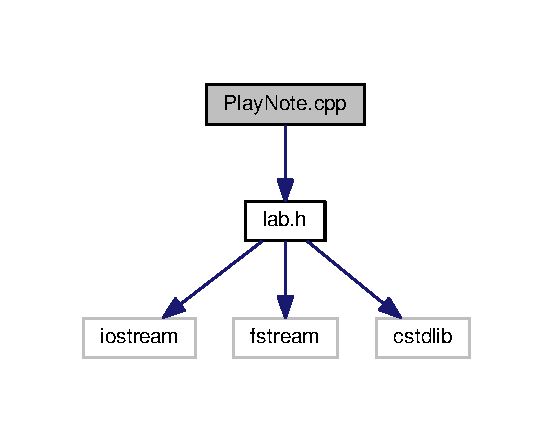
\includegraphics[width=265pt]{PlayNote_8cpp__incl}
\end{center}
\end{figure}
\subsubsection*{Functions}
\begin{DoxyCompactItemize}
\item 
void \hyperlink{PlayNote_8cpp_ad075a727cdddb38fe5bfa5d055e57161}{Play\+Note} (\hyperlink{structNOTE}{N\+O\+T\+E} \&note, float tempo)
\end{DoxyCompactItemize}


\subsubsection{Function Documentation}
\hypertarget{PlayNote_8cpp_ad075a727cdddb38fe5bfa5d055e57161}{\index{Play\+Note.\+cpp@{Play\+Note.\+cpp}!Play\+Note@{Play\+Note}}
\index{Play\+Note@{Play\+Note}!Play\+Note.\+cpp@{Play\+Note.\+cpp}}
\paragraph[{Play\+Note}]{\setlength{\rightskip}{0pt plus 5cm}void Play\+Note (
\begin{DoxyParamCaption}
\item[{{\bf N\+O\+T\+E} \&}]{note, }
\item[{float}]{tempo}
\end{DoxyParamCaption}
)}}\label{PlayNote_8cpp_ad075a727cdddb38fe5bfa5d055e57161}
This function plays the individual notes and fragments This creates a single string that the console can read as an instruction to play the note for a set duration 
\begin{DoxyCode}
8 \{
9     std::string s1 = \textcolor{stringliteral}{"play -qn synth "};
10     std::string s2 = \textcolor{stringliteral}{" pluck "};
11     
12     \textcolor{keywordtype}{string} ms = s1 + std::to\_string(note.\hyperlink{structNOTE_a258adf07267f95ab9630b33bad1b2fe2}{duration}/16.0) +
13                     s2 + note.\hyperlink{structNOTE_ae03dbb1306465fe61ec10da05fa5782e}{tone};
14         cout << ms << endl;
15         system(ms.c\_str());
16     
17     
18     
19 \}
\end{DoxyCode}

\hypertarget{pop_8cpp}{\subsection{pop.\+cpp File Reference}
\label{pop_8cpp}\index{pop.\+cpp@{pop.\+cpp}}
}
{\ttfamily \#include \char`\"{}lab.\+h\char`\"{}}\\*
Include dependency graph for pop.\+cpp\+:\nopagebreak
\begin{figure}[H]
\begin{center}
\leavevmode
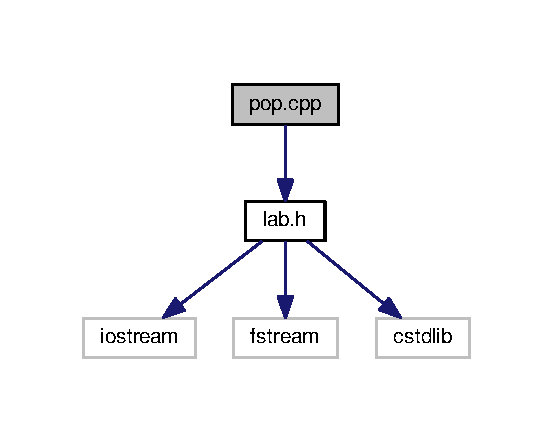
\includegraphics[width=265pt]{pop_8cpp__incl}
\end{center}
\end{figure}
\subsubsection*{Functions}
\begin{DoxyCompactItemize}
\item 
\hyperlink{lab_8h_a32c27cc471df37f4fc818d65de0a56c4}{S\+T\+A\+T\+U\+S} \hyperlink{pop_8cpp_a9ab82590ff3d7086853fd9b2106d255c}{Pop} (\hyperlink{structSTACK}{S\+T\+A\+C\+K} \&stack, int \&item)
\end{DoxyCompactItemize}


\subsubsection{Function Documentation}
\hypertarget{pop_8cpp_a9ab82590ff3d7086853fd9b2106d255c}{\index{pop.\+cpp@{pop.\+cpp}!Pop@{Pop}}
\index{Pop@{Pop}!pop.\+cpp@{pop.\+cpp}}
\paragraph[{Pop}]{\setlength{\rightskip}{0pt plus 5cm}{\bf S\+T\+A\+T\+U\+S} Pop (
\begin{DoxyParamCaption}
\item[{{\bf S\+T\+A\+C\+K} \&}]{stack, }
\item[{int \&}]{item}
\end{DoxyParamCaption}
)}}\label{pop_8cpp_a9ab82590ff3d7086853fd9b2106d255c}
This is a pop function it pos the elements off the top of the stack See inline comments for more clarification 
\begin{DoxyCode}
7 \{
8     \textcolor{keywordflow}{if} (stack.\hyperlink{structSTACK_a1b186cf876dace2f1e30fcbe260cad9a}{sp} == 0) \textcolor{comment}{//Check if stack is empty}
9         \textcolor{keywordflow}{return} \hyperlink{lab_8h_a32c27cc471df37f4fc818d65de0a56c4aecedb56d1405a60c6069f4a0139bdec5}{FAILED};
10     stack.\hyperlink{structSTACK_a1b186cf876dace2f1e30fcbe260cad9a}{sp}--; \textcolor{comment}{//decrement stack to the bottom element with stuff in it}
11     item = stack.\hyperlink{structSTACK_a6d512f82cbd75729347a293193039538}{buf}[stack.\hyperlink{structSTACK_a1b186cf876dace2f1e30fcbe260cad9a}{sp}]; \textcolor{comment}{// set a variable to equal what is in the element to use later}
12     
13     \textcolor{keywordflow}{return} \hyperlink{lab_8h_a32c27cc471df37f4fc818d65de0a56c4a2bc49ec37d6a5715dd23e85f1ff5bb59}{OK};
14 \}
\end{DoxyCode}

\hypertarget{push_8cpp}{\subsection{push.\+cpp File Reference}
\label{push_8cpp}\index{push.\+cpp@{push.\+cpp}}
}
{\ttfamily \#include \char`\"{}lab.\+h\char`\"{}}\\*
Include dependency graph for push.\+cpp\+:\nopagebreak
\begin{figure}[H]
\begin{center}
\leavevmode
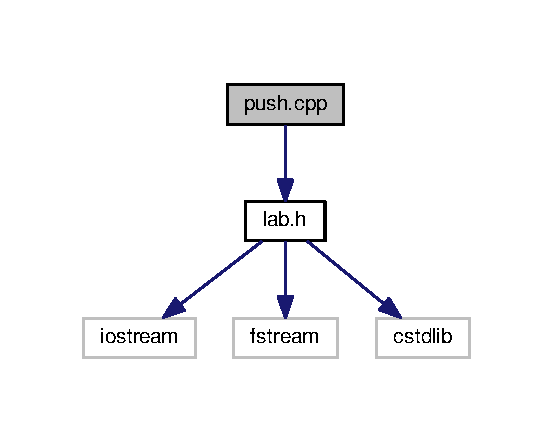
\includegraphics[width=265pt]{push_8cpp__incl}
\end{center}
\end{figure}
\subsubsection*{Functions}
\begin{DoxyCompactItemize}
\item 
\hyperlink{lab_8h_a32c27cc471df37f4fc818d65de0a56c4}{S\+T\+A\+T\+U\+S} \hyperlink{push_8cpp_a805a86f7ac8e643c87ea7d7cbb1b2c9c}{Push} (\hyperlink{structSTACK}{S\+T\+A\+C\+K} \&stack, int item)
\end{DoxyCompactItemize}


\subsubsection{Function Documentation}
\hypertarget{push_8cpp_a805a86f7ac8e643c87ea7d7cbb1b2c9c}{\index{push.\+cpp@{push.\+cpp}!Push@{Push}}
\index{Push@{Push}!push.\+cpp@{push.\+cpp}}
\paragraph[{Push}]{\setlength{\rightskip}{0pt plus 5cm}{\bf S\+T\+A\+T\+U\+S} Push (
\begin{DoxyParamCaption}
\item[{{\bf S\+T\+A\+C\+K} \&}]{stack, }
\item[{int}]{item}
\end{DoxyParamCaption}
)}}\label{push_8cpp_a805a86f7ac8e643c87ea7d7cbb1b2c9c}
This is the function to push the stack see the individual comments to understand it more 
\begin{DoxyCode}
7 \{
8     \textcolor{keywordflow}{if} (stack.\hyperlink{structSTACK_a1b186cf876dace2f1e30fcbe260cad9a}{sp} == stack.\hyperlink{structSTACK_ad10f9d8025122e8c82832d7a34c77e40}{size}) \textcolor{comment}{//check if the stack is full}
9         \textcolor{keywordflow}{return} \hyperlink{lab_8h_a32c27cc471df37f4fc818d65de0a56c4aecedb56d1405a60c6069f4a0139bdec5}{FAILED};
10     stack.\hyperlink{structSTACK_a6d512f82cbd75729347a293193039538}{buf}[stack.\hyperlink{structSTACK_a1b186cf876dace2f1e30fcbe260cad9a}{sp}] = item; \textcolor{comment}{// add the element into the empty space where the stack pointer was
       pointing}
11     stack.\hyperlink{structSTACK_a1b186cf876dace2f1e30fcbe260cad9a}{sp}++; \textcolor{comment}{//increment the stack pointer to add more into the stack}
12     \textcolor{keywordflow}{return} \hyperlink{lab_8h_a32c27cc471df37f4fc818d65de0a56c4a2bc49ec37d6a5715dd23e85f1ff5bb59}{OK};
13 \}
\end{DoxyCode}

\hypertarget{readSong_8cpp}{\subsection{read\+Song.\+cpp File Reference}
\label{readSong_8cpp}\index{read\+Song.\+cpp@{read\+Song.\+cpp}}
}
{\ttfamily \#include \char`\"{}lab.\+h\char`\"{}}\\*
Include dependency graph for read\+Song.\+cpp\+:\nopagebreak
\begin{figure}[H]
\begin{center}
\leavevmode
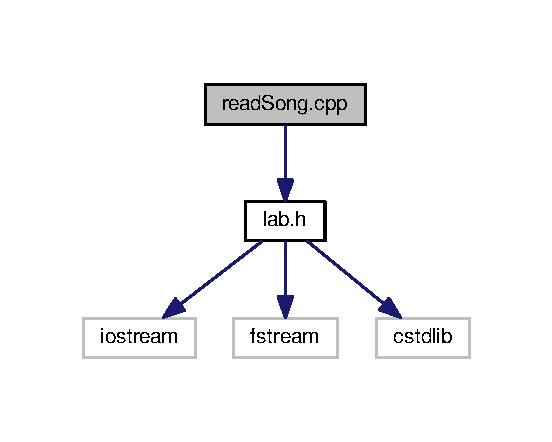
\includegraphics[width=265pt]{readSong_8cpp__incl}
\end{center}
\end{figure}
\subsubsection*{Functions}
\begin{DoxyCompactItemize}
\item 
void \hyperlink{readSong_8cpp_a7fac902a2930d3000a0b0a2788c09189}{readsong} (std\+::ifstream \&f, \hyperlink{structMUSICELMT}{M\+U\+S\+I\+C\+E\+L\+M\+T} m\mbox{[}$\,$\mbox{]}, int n)
\end{DoxyCompactItemize}


\subsubsection{Function Documentation}
\hypertarget{readSong_8cpp_a7fac902a2930d3000a0b0a2788c09189}{\index{read\+Song.\+cpp@{read\+Song.\+cpp}!readsong@{readsong}}
\index{readsong@{readsong}!read\+Song.\+cpp@{read\+Song.\+cpp}}
\paragraph[{readsong}]{\setlength{\rightskip}{0pt plus 5cm}void readsong (
\begin{DoxyParamCaption}
\item[{std\+::ifstream \&}]{f, }
\item[{{\bf M\+U\+S\+I\+C\+E\+L\+M\+T}}]{m\mbox{[}$\,$\mbox{]}, }
\item[{int}]{n}
\end{DoxyParamCaption}
)}}\label{readSong_8cpp_a7fac902a2930d3000a0b0a2788c09189}
This function reads the song as a whole It uses 2 indicators for readings a fragment or a note For note it takes in its tone and duration and for fragment it takes in its start and finish This function is read in main 
\begin{DoxyCode}
10 \{
11     \textcolor{keywordtype}{int} i = 0;
12     \textcolor{keywordtype}{char} type;
13     \textcolor{keywordflow}{while}(f>> type)
14      \{
15         \textcolor{keywordflow}{if}(type == \textcolor{charliteral}{'r'}) \{
16             f >> m[i].\hyperlink{structMUSICELMT_a662fdb18330107012ed8902725b08e5c}{note}.\hyperlink{structNOTE_ae03dbb1306465fe61ec10da05fa5782e}{tone} >> m[i].\hyperlink{structMUSICELMT_a662fdb18330107012ed8902725b08e5c}{note}.\hyperlink{structNOTE_a258adf07267f95ab9630b33bad1b2fe2}{duration};
17             m[i].\hyperlink{structMUSICELMT_aa9a541d279b1a98b190c1968217ad37f}{type} = \hyperlink{lab_8h_a41c816c739b4ab01c73879f01ae63880a3e1a299c993f58cef9ff1e4853051f02}{PLAYNOTE};
18         \}
19         \textcolor{keywordflow}{else} \textcolor{keywordflow}{if} (type == \textcolor{charliteral}{'f'}) \{
20             f >> m[i].\hyperlink{structMUSICELMT_ae418bce8087e7510ad8563a87b4c1c63}{fragment}.\hyperlink{structFRAGMENT_a9a2c77dc5f1c259a9a063f8e6ae18724}{start} >> m[i].\hyperlink{structMUSICELMT_ae418bce8087e7510ad8563a87b4c1c63}{fragment}.
      \hyperlink{structFRAGMENT_a3edee1f345e206cdc220b16d7d290018}{finish};
21             m[i].\hyperlink{structMUSICELMT_aa9a541d279b1a98b190c1968217ad37f}{type} = \hyperlink{lab_8h_a41c816c739b4ab01c73879f01ae63880a0fab3b3b81cc5ad4ac6d6b74b50869e5}{PLAYFRAGMENT};
22     \}
23     i++;
24 \}
25     
26     m[i].\hyperlink{structMUSICELMT_aa9a541d279b1a98b190c1968217ad37f}{type} = \hyperlink{lab_8h_a41c816c739b4ab01c73879f01ae63880a2175f634cdffa7045d36d1b0cca00ed4}{PLAYSTOP};
27 \}
\end{DoxyCode}

\hypertarget{specification_8dox}{\subsection{specification.\+dox File Reference}
\label{specification_8dox}\index{specification.\+dox@{specification.\+dox}}
}

%--- End generated contents ---

% Index
\newpage
\phantomsection
\addcontentsline{toc}{section}{Index}
\printindex

\end{document}
